\chapter{Introduction}
Over recent years, The study of neutron-rich nuclei has increasing attention in the field of nuclear physics, providing invaluable insights into the conventional nuclear models and interactions in the condition far from stable nuclei. One particularly intriguing subclass is neutron halo nuclei\cite{Tanihata96}, which feature an extended halo of one or two loosely bound neutrons far from its core. The first discovery of neutron halo nuclei was ${}^{11}$Li by I. Tanihata et al\cite{Tanihata85}. In Figure 1.1, ${}^{11}$Li has enormously large radius compared to neighboring  He, Li, Be and C isotopes which has similar A number. Based on this discovery, he suggested that ${}^{11}$Li has a large deformation or a long tail in matter distribution. After that, P. G. Hansen and B. Jonson\cite{HansenandJonson} suggested ${}^{11}$Li as a neutron halo nuclei due to the large neutron radius compared to its core ${}^{9}$Li.

\begin{figure}
    \centering
    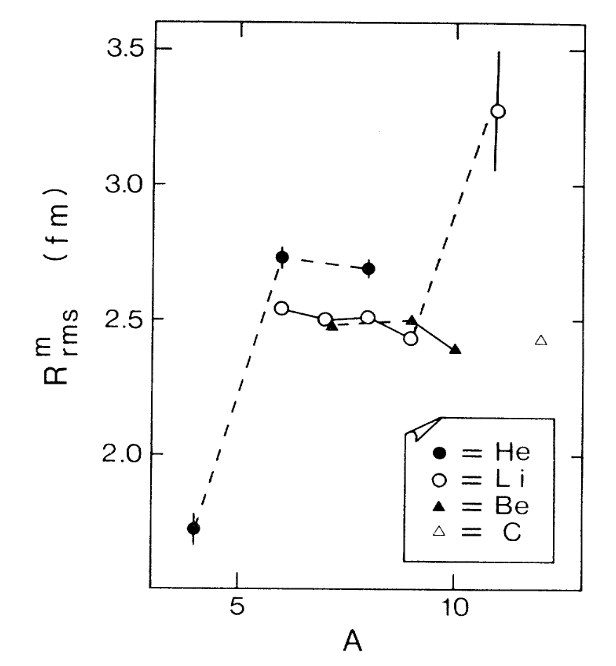
\includegraphics[width=7cm]{chapter1/Radius_of_11Li.png}
    \caption{Matter rms radius of He, Li, Be and C isotopes. ${}^{11}$Li has significantly large radius compared to other Li isotopes.}
\end{figure}

After more research on this theme, many people suggested how to decide a nuclei as a halo nuclei. One is obviously a small neutron separation energy. Compared to common separation energy of stable nuclei 6 - 8MeV, many neutron rich nuclei have extremely small separation energy less than 1 MeV. And because of this, the halo nuclei usually have large radius. Given that the neutron wavefunction is a square well potential, the wavefunction of neutron can be written as
\begin{align}
    \Psi(r) = \bigg(\frac{2\pi}{k}\bigg)\bigg(\frac{-e^{k r}}{r}\bigg)\bigg[\frac{e^{k R}}{(1+ k R)^{1/2}}\bigg],
\end{align}
where R is the width of the potential. With this wavefunction, the density distribution of the neutron is
\begin{align}
    \rho(r) = |\Psi(r)|^2 \propto \frac{e^{-2k r}}{r^2}.
\end{align}
The factor $k$ determines the tail of the neutron, and it is related to the neutron separation energy by
\begin{align}
    (\hbar k)^2 = 2\mu S_n,
\end{align}
where $\mu$ is the effective mass of system and $S_n$ is the neutron separation energy. From this equation, we can see that the $k$ is inversely proportional to the neutron separation energy. So, the smaller the neutron separation energy is, the larger the $k$ is. And the larger the $k$ is, the longer tail of neutron is. So, the halo nuclei usually have small neutron separation energy and large radius.

% halo feature 2
The narrow momentum distribution is also the feature of halo nuclei. The momentum distribution of neutron [$f (p)$] can be expressed by the Fourier transform of the wavefunction (1.1),
\begin{align}
    f(p) = \frac{C}{p^2+(\hbar k)^2} %C / (p^2 + k^2), 
\end{align}
where $p$ is the momentum of the neutron and the width of the distribution is defined by $k$ which related with separation energy. In this formula, the concept of Heigenberg uncertainty principle is shown. The smaller the $k$, the wider the density distribution, and also the narrower the momentum distribution is. 

% halo feature 3
Another parameter which define a halo nuclei is the orbital angular momentum of valance neutron. The shape of momentum distribution depends on not only the separation energy, but also the angular momentum ($l$) of the orbital. The width of The centrifugal barrier which proportional to $l(l+1)/r^2$ largely affect the density distribution of neutron. 
%Also in three-body halo system, the centrifugal barrier is defined in the form of $[(K+3/2)(K+5/2)]/\rho^2$ by Fedorov et al.\cite{fedorov} with the quantum number $K$ (usually called hypermomenent). In this formula, the hight of centrifugal barrier rapidly increases with $K$. Ad even $K = 0$ has centrifugal barr

low orbital angular momentum of valance neutron makes the halo nuclei.

% halo feature 4
The most important feature of a halo nucleus focused on this research is soft mode of electric dipole excitation. Given that halo nuclei has a core and loosely bounded valance neutron, the core and valance neutron can be polarized by the external electric field. And this dipole excitation mode is shown in very low energy region, because the halo structure response easily to the external electric field. This soft mode of electric dipole excitation is called Soft E1 excitation. This feature predicted by Hansen and Jonse\cite{HansenandJonson}, and also Ikeda et al.\cite{Ikeda}.

In E1 reduced transition probability, the term 'reduced' means that the transition matrix element is independent of the magnetic substate of the initial and final states. The E1 reduced transition probability is defined as
\begin{align}
    B(E1) = \frac{|\langle \Phi_f ||\hat{T}(E1)|| \Phi_i\rangle|^2}{(2J_i + 1)},
\end{align}

In boron isotopes, the soft E1 excitation of ${}^{19}$B is observed by K. J. Cook et al.\cite{KJCook} using Coulomb dissociation method. (result briefly)


\begin{figure}[t]
    \centering
    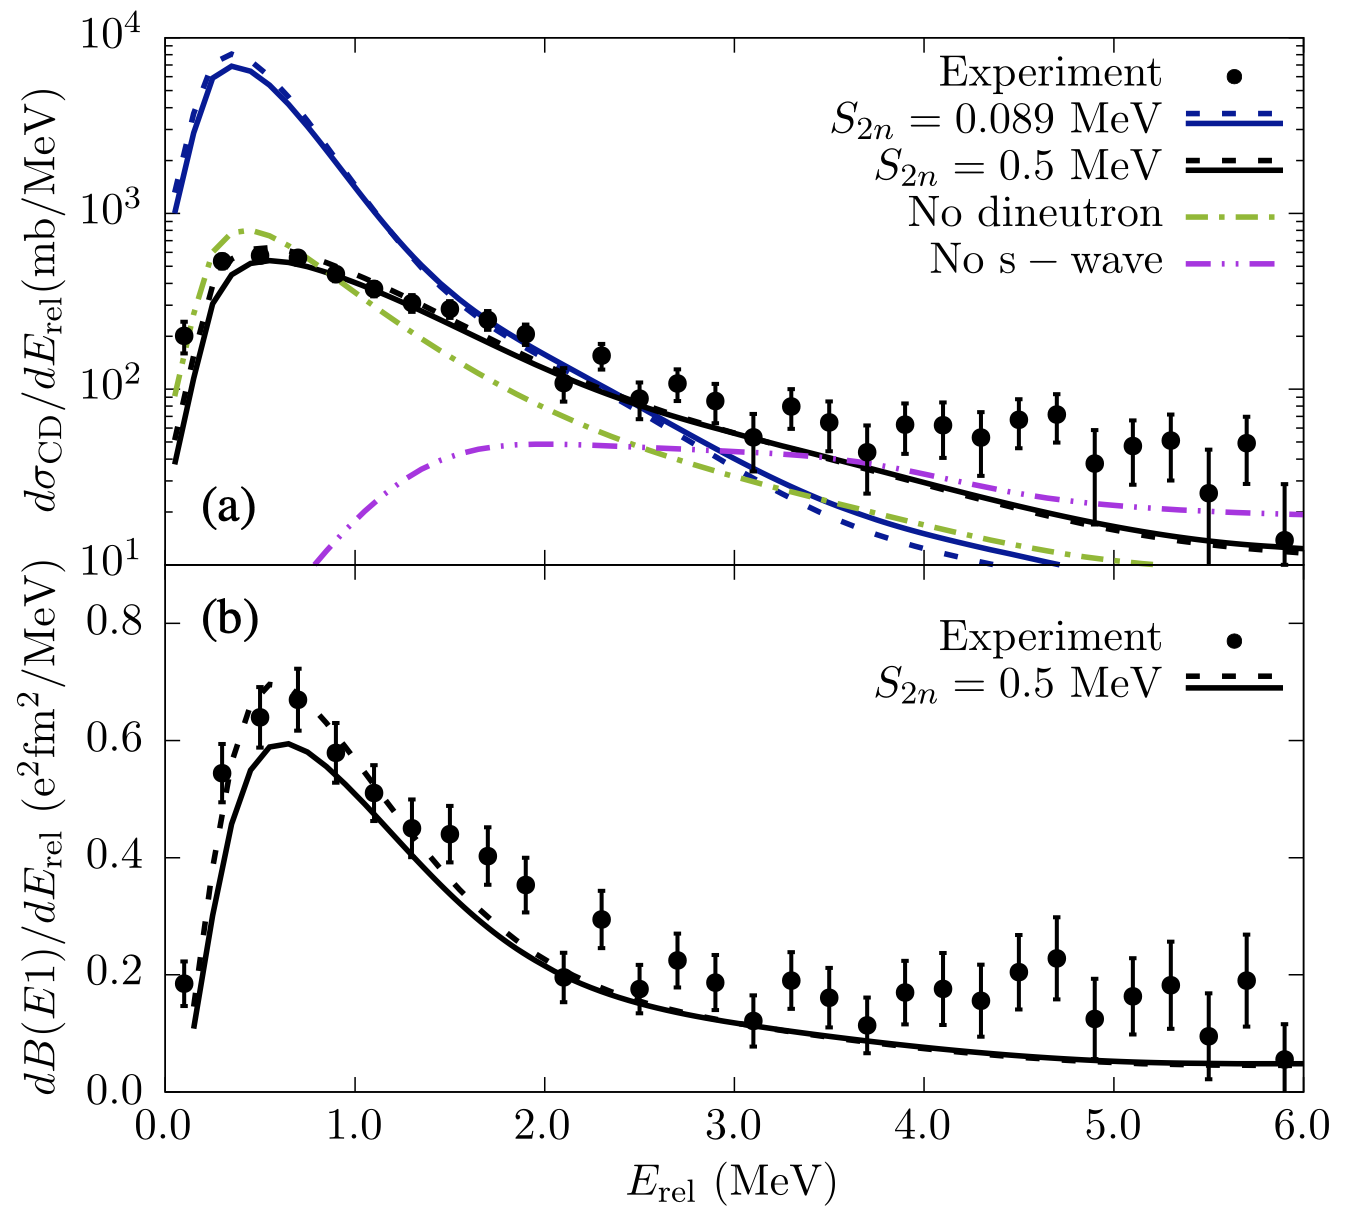
\includegraphics[width=10cm]{chapter1/19B_B(E1).png}
    \caption{The B(E1) distribution of ${}^{19}$B. The peak at 0.5 MeV is the soft E1 excitation.}
\end{figure}

But how to define halo nuclei is still in debate. Because there is no clear definition what separation energy halo nuclei should have, or what radius halo nuclei should have. And the mixture between several orbital angular momentum of valance neutron makes the situation even more difficult to interpret. For example, 

One example is two neutron halo nuclei in boron isotope, ${}^{17}$B and ${}^{19}$B. The first study about these nuclei was performed by T. Suzuki et al\cite{suzuki99}. They measure the reaction cross section of boron isotope and extracted the matter radius of them. 

\begin{figure}
        \centering
        %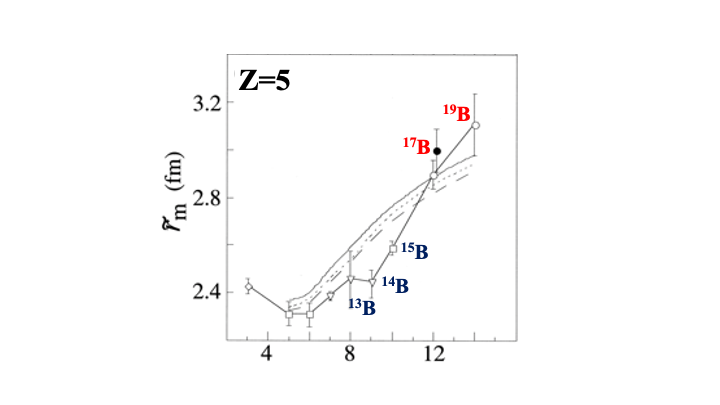
\includegraphics[width=14cm]{chapter1/Radius_of_boron.png}
    \end{figure}

But there were many discussion between the structures of 2-neutron halo nuclei of Boron isotopes. T. Suzuki et al. assumed that both ${}^{17}B$ and ${}^{19}$B is 2-neutron halo nuclei, due to the large radius of both ${}^{17}$B and ${}^{19}$B. But he also suggested ${}^{19}$B is hindered 2-neutron halo nuclei due to the small ratio between halo and core radius.


\begin{align}
    \Psi({}^{19}\text{B}) = \psi({}^{17}\text{B}) \otimes [\alpha |1d_{5/2} \rangle^2 + \beta |2s_{1/2} \rangle^2]    
\end{align}

\begin{figure}
    \centering
    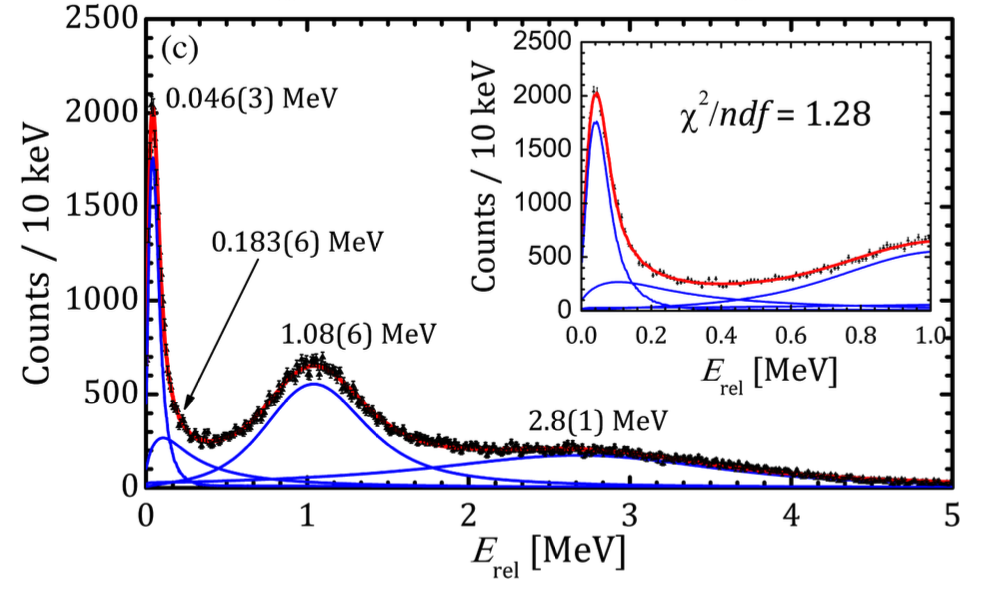
\includegraphics[width=10cm]{chapter1/17B_ZHYang.png}
\end{figure}
But recently, Z. H. Yang et al. \cite{ZHYang} shows a strong evidence that ${}^{17}$B might not be a two neutron halo nuclei. He performed the quasi-free ($p,pn$) scattering reaction and extracted the relative energy distribution of ${}^{16}$B. He assumed that the knocked-out neutron from the ${}^{17}$B  should almost come from $1d_{5/2}$ or $2s_{1/2}$ orbital and got the relative energy distribution of ${}^{16}$B. (Figure 1.3) 
And also, he obtained the spectroscopic factors for $1d_{5/2}$ and $2s_{1/2}$ orbital and there was surprisingly small percentage 9(2)\% of $2s_{1/2}$ orbital. This result is very different from the ones, which are 36(19)\%, 69(20)\%, 50(10)\% and by T. Suzuki and Y. Yamaguchi.

Also Estradé et al. \cite{Estrade} suggested there is a
\\
So, in this research, we study the Soft E1 excitation of ${}^{17}$B, which can be the final key for deciding ${}^{17}$B as a halo nuclei or not. In this thesis, we will discuss the Coulomb Dissociation of ${}^{17}$B as a tool for searching the Soft E1 excitation of ${}^{17}$B. 

\begin{align}
    \Psi({}^{17}\text{B}) = \psi({}^{15}\text{B}) \otimes [\alpha |1d_{5/2} \rangle^2 + \beta |2s_{1/2} \rangle^2]
\end{align}

\begin{align}
    \langle \text{cos} \theta_{nn} \rangle &= \langle \Psi({}^{11}\text{Li}) | \text{cos} \theta_{nn} | \Psi({}^{11}\text{Li}) \rangle \notag \\
    &= \alpha^2 \langle (1d_{5/2})^2 | \text{cos} \theta_{nn} | (1d_{5/2})^2 \rangle + \beta^2 \langle (2s_{1/2})^2 | \text{cos} \theta_{nn} | (2s_{1/2})^2 \rangle \notag \\
    &\hspace{4mm} + 2\alpha \beta \langle (1d_{5/2})^2 | \text{cos} \theta_{nn} | (2s_{1/2})^2 \rangle \notag \\
    &= 2\alpha \beta \langle (1d_{5/2})^2 | \text{cos} \theta_{nn} | (2s_{1/2})^2 \rangle
\end{align}

where $|(1d_{5/2}^2)$ represents $|\psi({}^{15}\text{B})\otimes|$
